\documentclass[12pt,oneside]{report}
\usepackage{graphicx}
\usepackage{epstopdf}
\usepackage{fancyhdr}
\usepackage{tabularx}
\usepackage{mathrsfs,amsmath}
\usepackage[table]{xcolor}
\newcommand{\gammabar}{\ensuremath\gamma\kern-0.88em-}
%some decoration for black cell tabular
\newcommand\BlackCell[1]{%
  \multicolumn{1}{c}{\cellcolor{black}\textcolor{white}{#1}}
}
\usepackage{pgf,tikz}
\usetikzlibrary{patterns}
\usetikzlibrary{arrows}
\newcommand*\circled[1]{\tikz[baseline=(char.base)]{
            \node[shape=circle,draw,thick,inner sep=0pt,minimum size=17pt] (char) {#1};}}
%creating fancy header and footer
\fancyhf{}
\lhead{Medical Imaging}
\chead{Homework 3}
\rhead{P.H.An-9651}
\cfoot{\thepage}
%font=default,size 12pt
%Configure page layout: a4, margin 0.79in, onesided, indent 0.5in
\paperwidth=8.27in
\paperheight=11.69in
\voffset=-0.21in
\hoffset=-0.21in
\oddsidemargin=0in
\evensidemargin=0in
\topmargin=-23pt
\headheight=12pt
\headsep=25pt
\marginparsep=0in
\marginparwidth=0in
\footskip=30pt
\marginparpush=0in
\textwidth=6.69in
\textheight=9.61in
%indent of a first line of new paragraphc is 0.5in to use \indent or \par
\parindent=0.5in
%set distance btw lines
\baselineskip=0pt
%set disctance btw pars
\parskip=0pt
%create a listing environment for arranging text
%tree level 1: {\textbullet}{0in}{0in}{\parindent}
%tree level 2: dependent :D
\newenvironment{tree}[6]{
\begin{list}{#1}{\parskip=0in \topsep=#5 \itemsep=#6 \parsep=0in \partopsep=0in \leftmargin=#2 \rightmargin=#3 \itemindent=#4 \listparindent=\itemindent}
}{\end{list}}
%creat a small section document :D
\newenvironment{ssection}[7]{
\framebox{\textbf{#1}} \textbf{#2}
\begin{tree}{#3}{#4}{#5}{\parindent}{#6}{#7}
}{\end{tree}}
%fix other errors manually if needed: line break, etc.
\begin{document} %SINUSOIDAL STEADY-STATE ANALYSIS
\thispagestyle{plain}
\pagestyle{fancy}
\noindent
\begin{tabular}{c}
\BlackCell{\parbox{\textwidth}{}}\\
\BlackCell{\parbox{\textwidth}{\centerline{{\Large \textbf{\emph{Homework 3}}}}}}\\
\BlackCell{\parbox{\textwidth}{}}\\
\end{tabular}
\begin{flushright}
\large \textit{Phan Hoang An - 9651}
\end{flushright}
\ \\
\begin{ssection}{Problem 5.12}{}{}{0in}{0in}{0pt}{0pt}
\item 
\begin{center}
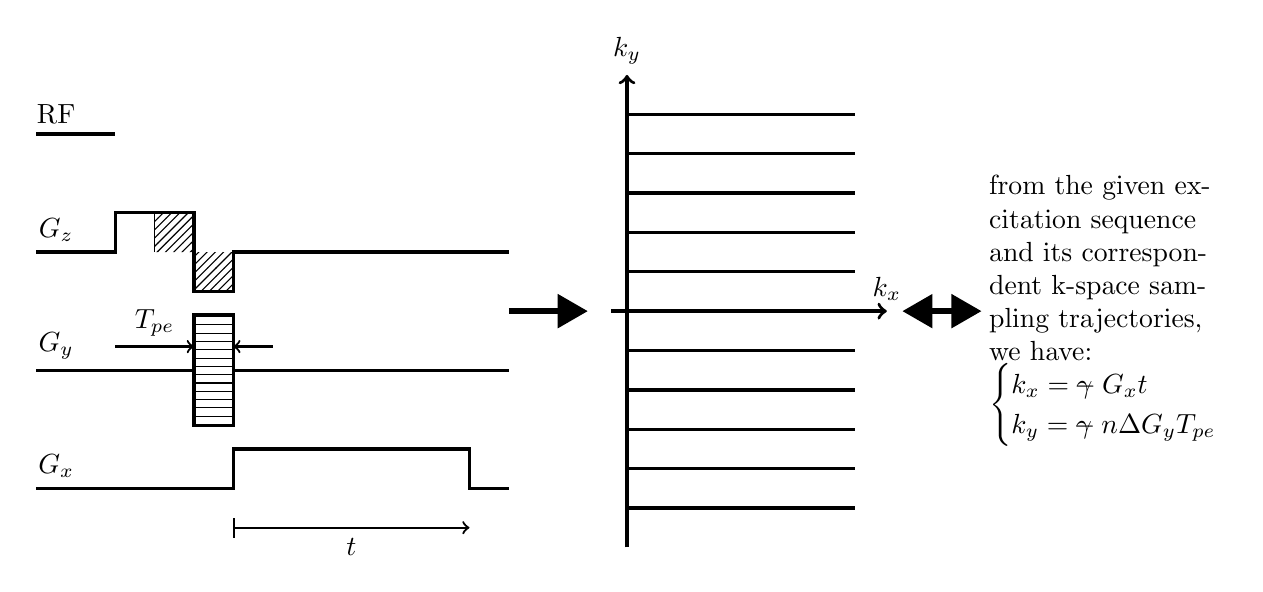
\begin{tikzpicture}[scale=1]
\draw[very thick] (0,0) -- node[near start,above]{RF} (1,0);
\pgftransformxshift{1.5cm}
\draw[very thick] plot[smooth] file {sinc.txt} -- ++(4,0);
\pgftransformshift{\pgfpoint{-1.5cm}{-1.5cm}}
\draw[very thick] (0,0) -- node[near start,above]{$G_z$} (1,0) 
-- (1,0.5) -- (2,0.5) -- (2,-0.5) -- (2.5,-0.5) -- (2.5,0) -- ++(3.5,0);
\filldraw[pattern=north east lines] (1.5,0) 
-- (1.5,0.5) -- (2,0.5) -- (2,-0.5) -- (2.5,-0.5) -- (2.5,0);
\pgftransformshift{\pgfpoint{0cm}{-1.5cm}}
\draw[very thick] (0,0) -- node[near start,above]{$G_y$} (1,0) -- (2,0) (2.5,0) -- (6,0);
\filldraw[pattern=horizontal lines,line width=1.2pt] (2,-0.7) rectangle (2.5,0.7);
\draw[thick,->] (1,0.3) -- node[midway,above]{$T_{pe}$} (2,0.3);
\draw[thick,->] (3,0.3) -- (2.5,0.3);
\pgftransformshift{\pgfpoint{0cm}{-1.5cm}} 
\draw[very thick] (0,0) -- node[near start,above]{$G_x$} (1,0) -- (2,0) -- (2.5,0)
-- (2.5,0.5) -- (5.5,0.5) -- (5.5,0) -- ++(0.5,0); 
\draw[thick,|->] (2.5,-0.5) -- node[midway,below]{$t$} (5.5,-0.5);
\pgftransformshift{\pgfpoint{6cm}{2.25cm}} 
\draw[-triangle 60,line width=2pt] (0,0) -- (1,0);
\pgftransformshift{\pgfpoint{1.5cm}{0cm}}
\draw[very thick,->] (-0.2,0) -- (3.3,0) node[anchor=south]{$k_x$};
\draw[very thick,->] (0,-3) -- (0,3) node[anchor=south]{$k_y$};
\foreach \y in {-2.5,-2,...,2.5} \draw[very thick] (0,\y) -- (2.9,\y);
\pgftransformshift{\pgfpoint{3.5cm}{0cm}}
\draw[triangle 60-triangle 60,line width=2pt] (0,0) -- (1,0);
\pgftransformshift{\pgfpoint{1.1cm}{0cm}}
\node at (1.5,0) [text width=3cm] {
from the given excitation sequence and its correspondent k-space sampling trajectories, we have:\\
$
\begin{cases}
k_x=\displaystyle\gammabar G_x t\\
k_y=\displaystyle\gammabar n \Delta G_y T_{pe}
\end{cases}
$
};
\end{tikzpicture}
\end{center}
\item To have the FID signals that will generate the k-space coverage in the left half plane along $k_x$ direction, we need to reverse the current direction of the $\vec{G}_x$ gradient field. To illustrate,
\begin{center}
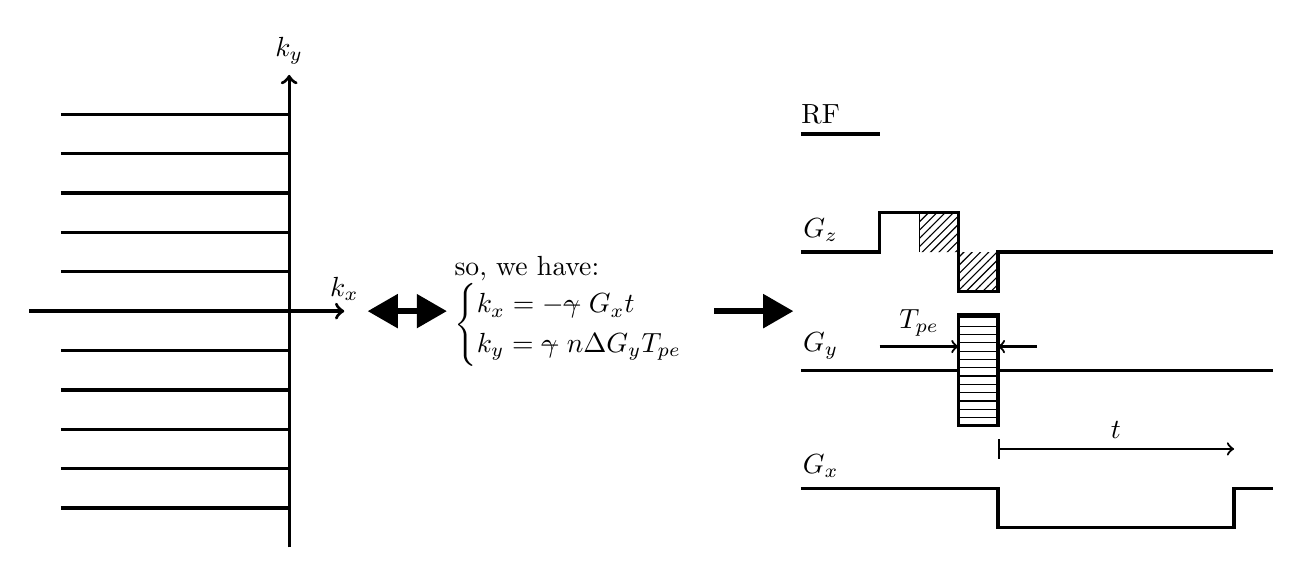
\begin{tikzpicture}[scale=1]
\draw[very thick,->] (-3.3,0) -- (0.7,0) node[anchor=south]{$k_x$};
\draw[very thick,->] (0,-3) -- (0,3) node[anchor=south]{$k_y$};
\foreach \y in {-2.5,-2,...,2.5} \draw[very thick] (-2.9,\y) -- (0,\y);
\pgftransformshift{\pgfpoint{1cm}{0cm}}
\draw[triangle 60-triangle 60,line width=2pt] (0,0) -- (1,0);
\pgftransformshift{\pgfpoint{1.1cm}{0cm}}
\node at (1.5,0) [text width=3cm] {
so, we have:\\
$
\begin{cases}
k_x=-\displaystyle\gammabar G_x t\\
k_y=\displaystyle\gammabar n \Delta G_y T_{pe}
\end{cases}
$
};
\pgftransformshift{\pgfpoint{3.3cm}{0cm}}
\draw[-triangle 60,line width=2pt] (0,0) -- (1,0);
\pgftransformshift{\pgfpoint{1.1cm}{2.25cm}} 
\draw[very thick] (0,0) -- node[near start,above]{RF} (1,0);
\pgftransformxshift{1.5cm}
\draw[very thick] plot[smooth] file {sinc.txt} -- ++(4,0);
\pgftransformshift{\pgfpoint{-1.5cm}{-1.5cm}}
\draw[very thick] (0,0) -- node[near start,above]{$G_z$} (1,0) 
-- (1,0.5) -- (2,0.5) -- (2,-0.5) -- (2.5,-0.5) -- (2.5,0) -- ++(3.5,0);
\filldraw[pattern=north east lines] (1.5,0) 
-- (1.5,0.5) -- (2,0.5) -- (2,-0.5) -- (2.5,-0.5) -- (2.5,0);
\pgftransformshift{\pgfpoint{0cm}{-1.5cm}}
\draw[very thick] (0,0) -- node[near start,above]{$G_y$} (1,0) -- (2,0) (2.5,0) -- (6,0);
\filldraw[pattern=horizontal lines,line width=1.2pt] (2,-0.7) rectangle (2.5,0.7);
\draw[thick,->] (1,0.3) -- node[midway,above]{$T_{pe}$} (2,0.3);
\draw[thick,->] (3,0.3) -- (2.5,0.3);
\pgftransformshift{\pgfpoint{0cm}{-1.5cm}} 
\draw[very thick] (0,0) -- node[near start,above]{$G_x$} (1,0) -- (2,0) -- (2.5,0)
-- (2.5,-0.5) -- (5.5,-0.5) -- (5.5,0) -- ++(0.5,0); 
\draw[thick,|->] (2.5,0.5) -- node[midway,above]{$t$} (5.5,0.5);
\end{tikzpicture}
\end{center}
\end{ssection}
\newpage\noindent
\begin{ssection}{Problem 5.14}{}{}{0in}{0in}{7pt}{0pt}
\item A gradient-echo imaging sequence with rectilinear sampling of k-space
\begin{center}
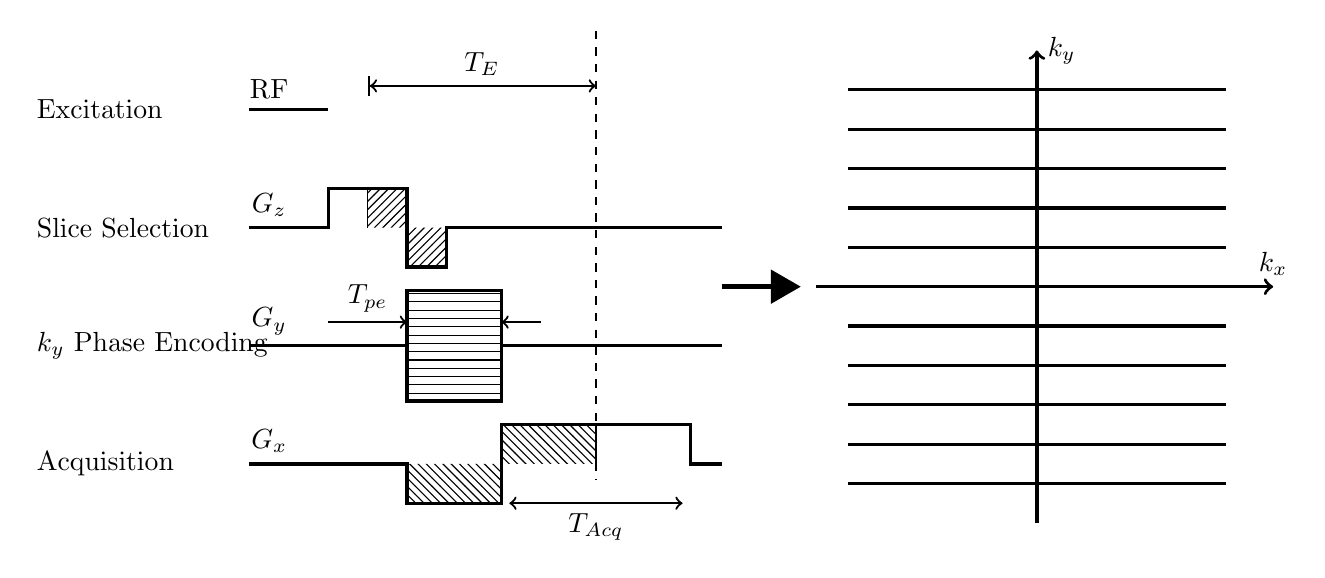
\begin{tikzpicture}[scale=1]
\node at (1.5,0) [text width=3cm] {Excitation};
\node at (1.5,-1.5) [text width=3cm] {Slice Selection};
\node at (1.5,-3) [text width=3cm] {$k_y$ Phase \mbox{Encoding}};
\node at (1.5,-4.5) [text width=3cm] {Acquisition};
\pgftransformshift{\pgfpoint{2.7cm}{0cm}}
\draw[very thick] (0,0) -- node[near start,above]{RF} (1,0);
\draw[thick,|<->] (1.5,0.3) -- node[midway,above]{$T_E$} (4.4,0.3);
\draw[semithick,dashed] (4.4,1) -- (4.4,-4.7);
\pgftransformxshift{1.5cm}
\draw[very thick] plot[smooth] file {sinc.txt} -- ++(4,0);
\pgftransformshift{\pgfpoint{-1.5cm}{-1.5cm}}
\draw[very thick] (0,0) -- node[near start,above]{$G_z$} (1,0) 
-- (1,0.5) -- (2,0.5) -- (2,-0.5) -- (2.5,-0.5) -- (2.5,0) -- ++(3.5,0);
\filldraw[pattern=north east lines] (1.5,0) 
-- (1.5,0.5) -- (2,0.5) -- (2,-0.5) -- (2.5,-0.5) -- (2.5,0);
\pgftransformshift{\pgfpoint{0cm}{-1.5cm}}
\draw[very thick] (0,0) -- node[near start,above]{$G_y$} (1,0) -- (2,0) (3.2,0) -- (6,0);
\filldraw[pattern=horizontal lines,line width=1.2pt] (2,-0.7) rectangle (3.2,0.7);
\draw[thick,->] (1,0.3) -- node[midway,above]{$T_{pe}$} (2,0.3);
\draw[thick,->] (3.7,0.3) -- (3.2,0.3);
\pgftransformshift{\pgfpoint{0cm}{-1.5cm}} 
\draw[very thick] (0,0) -- node[near start,above]{$G_x$} (1,0) -- (2,0)
-- (2,-0.5) -- (3.2,-0.5) -- (3.2,0.5) -- (5.6,0.5) -- (5.6,0) -- (6,0);
\filldraw[pattern=north west lines] (2,0)
-- (2,-0.5) -- (3.2,-0.5) -- (3.2,0.5) -- (4.4,0.5) -- (4.4,0);
\draw[thick,<->] (3.3,-0.5) -- node[midway,below]{$T_{Acq}$} (5.5,-0.5);
\pgftransformshift{\pgfpoint{6cm}{2.25cm}} 
\draw[-triangle 60,line width=2pt] (0,0) -- (1,0);
\pgftransformshift{\pgfpoint{4cm}{0cm}}
\draw[very thick,->] (-2.8,0) -- (3,0) node[anchor=south]{$k_x$};
\draw[very thick,->] (0,-3) -- (0,3) node[anchor=west]{$k_y$};
\foreach \y in {-2.5,-2,...,2.5} \draw[very thick] (-2.4,\y) -- (2.4,\y);
\end{tikzpicture}
\end{center}
\end{ssection}
\begin{ssection}{Problem 5.16}{}{}{0in}{0in}{7pt}{0pt}
\item The following spin-echo imaging sequence builds the given $k'$-space sampling trajectories.
\begin{center}
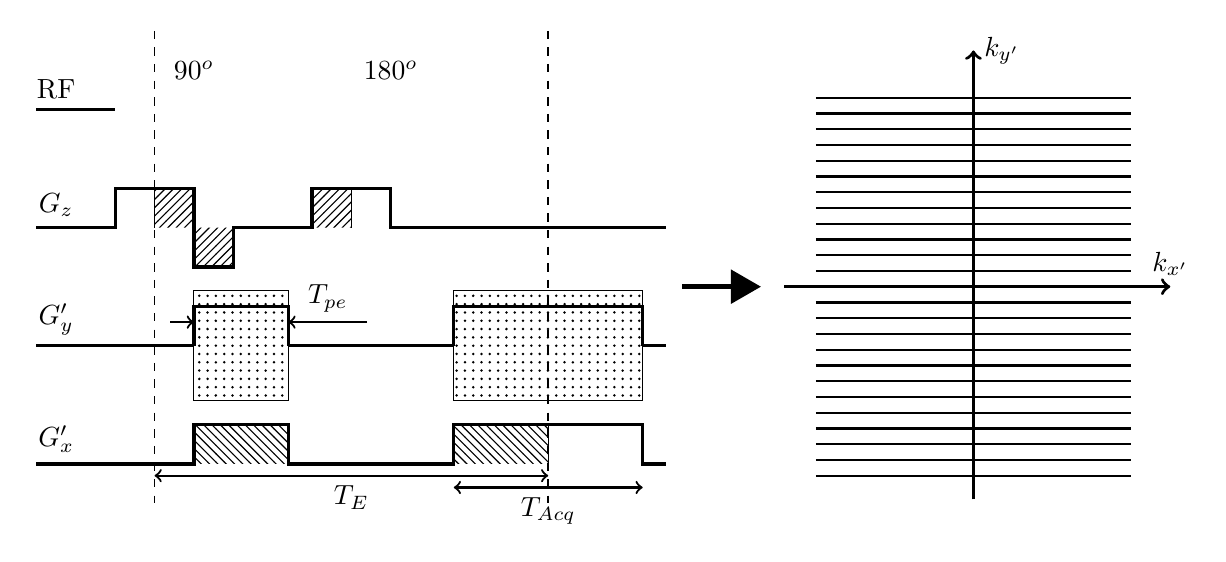
\begin{tikzpicture}[scale=1]
\draw[very thick] (0,0) -- node[near start,above]{RF} (1,0); 
\draw[semithick,dashed] (6.5,1) -- (6.5,-5) (1.5,1) -- (1.5,-5);
\pgftransformxshift{1.5cm}
\draw[very thick] plot[smooth] file {sincsmall.txt} -- (2,0);
\node at (0.5,0.5) [] {$90^o$};
\pgftransformxshift{2.5cm}
\draw[very thick] plot[smooth] file {sinc.txt} -- (4,0);
\node at (0.5,0.5) [] {$180^o$};
\pgftransformshift{\pgfpoint{-4cm}{-1.5cm}}
\draw[very thick] (0,0) -- node[near start,above]{$G_z$} (1,0) 
-- (1,0.5) -- (2,0.5) -- (2,-0.5) -- (2.5,-0.5) -- (2.5,0) 
-- (3.5,0) -- (3.5,0.5) -- (4.5,0.5) -- (4.5,0) -- (8,0);
\filldraw[pattern=north east lines] (1.5,0) 
-- (1.5,0.5) -- (2,0.5) -- (2,-0.5) -- (2.5,-0.5) -- (2.5,0) (3.5,0) -- (3.5,0.5) -- (4,0.5) -- (4,0);
\pgftransformshift{\pgfpoint{0cm}{-1.5cm}}
\draw[very thick] (0,0) -- node[near start,above]{$G_y'$} (1,0) -- (2,0) (3.2,0) -- (5.3,0) (7.7,0) -- (8,0);
\draw[very thick] (2,0) -- (2,0.5) -- (3.2,0.5) -- (3.2,0) (5.3,0) -- (5.3,0.5) -- (7.7,0.5) -- (7.7,0);
\filldraw[pattern=dots] (2,-0.7) rectangle (3.2,0.7) (5.3,-0.7) rectangle (7.7,0.7);
\draw[thick,->] (1.7,0.3) -- (2,0.3);
\draw[thick,->] (4.2,0.3) -- node[midway,above]{$T_{pe}$} (3.2,0.3);
\pgftransformshift{\pgfpoint{0cm}{-1.5cm}} 
\draw[very thick] (0,0) -- node[near start,above]{$G_x'$} (1,0) -- (2,0)
-- (2,0.5) -- (3.2,0.5) -- (3.2,0) -- (5.3,0) -- (5.3,0.5) -- (7.7,0.5) -- (7.7,0) -- (8,0);
\filldraw[pattern=north west lines] (2,0)
-- (2,0.5) -- (3.2,0.5) -- (3.2,0) (5.3,0) -- (5.3,0.5) -- (6.5,0.5) -- (6.5,0);
\draw[thick,<->] (5.3,-0.3) -- node[midway,below]{$T_{Acq}$} (7.7,-0.3);
\draw[thick,<->] (1.5,-0.15) -- node[midway,below]{$T_{E}$} (6.5,-0.15);
\pgftransformshift{\pgfpoint{8.2cm}{2.25cm}} 
\draw[-triangle 60,line width=2pt] (0,0) -- (1,0);
\pgftransformshift{\pgfpoint{3.7cm}{0cm}}
\draw[very thick,->] (-2.4,0) -- (2.5,0) node[anchor=south]{$k_{x'}$};
\draw[very thick,->] (0,-2.7) -- (0,3) node[anchor=west]{$k_{y'}$};
\foreach \y in {-2.4,-2.2,...,2.4} \draw[thick] (-2,\y) -- (2,\y);
\end{tikzpicture}
\end{center}
\begin{center}
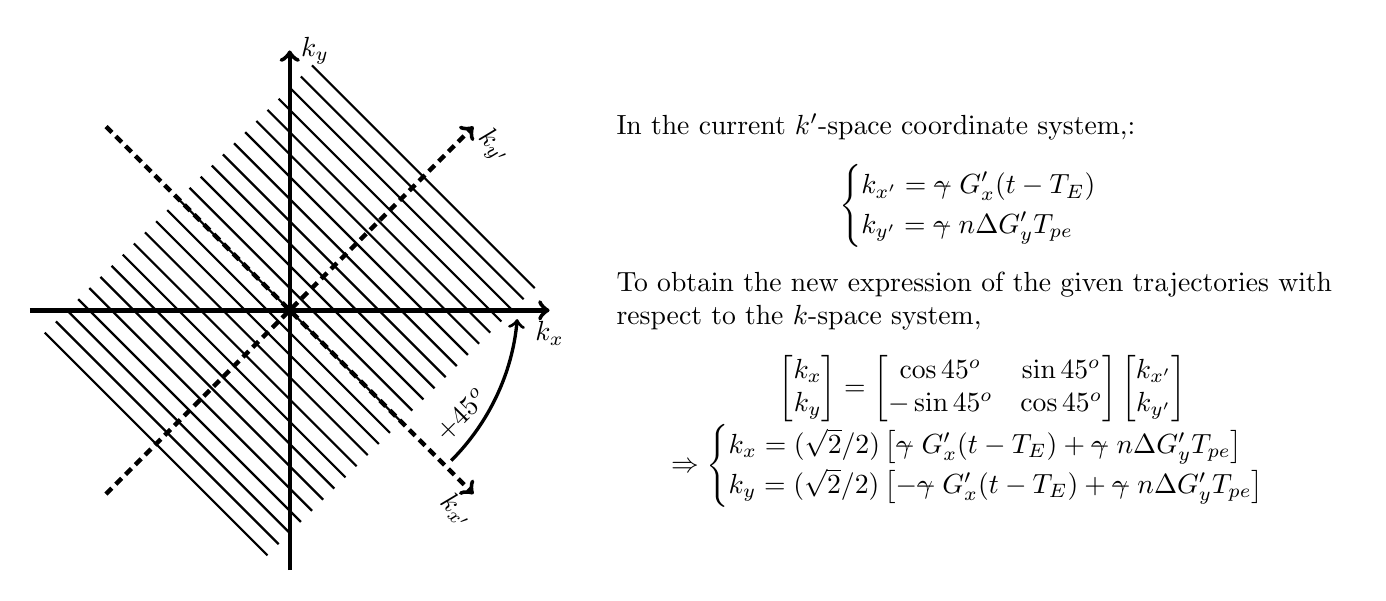
\begin{tikzpicture}[scale=1]
\pgftransformshift{\pgfpoint{3.3cm}{0cm}}
\draw[ultra thick,->] (-3.3,0) -- (3.3,0) node[anchor=north]{$k_x$};
\draw[ultra thick,->] (0,-3.3) -- (0,3.3) node[anchor=west]{$k_y$};
\pgftransformrotate{-45}
\draw[densely dashed,ultra thick,->] (-3.3,0) -- (3.3,0) node[rotate=-45,anchor=north]{$k_{x'}$};
\draw[densely dashed,ultra thick,->] (0,-3.3) -- (0,3.3) node[rotate=-45,anchor=west]{$k_{y'}$};
\foreach \y in {-2.4,-2.2,...,2.4} \draw[thick] (-2,\y) -- (2,\y);
\draw[very thick,->] (2.8,0.1) arc (0:40:2.9) node[rotate=45,near start,above]{$+45^o$};
\pgftransformrotate{45}
\pgftransformshift{\pgfpoint{8.8cm}{0cm}}
\node at (0,0) [text width=9.3cm] {
In the current $k'$-space coordinate system,:
\begin{center}
$
\begin{cases}
k_{x'}=\displaystyle\gammabar G_x' (t-T_E)\\
k_{y'}=\displaystyle\gammabar n \Delta G_y' T_{pe}
\end{cases}
$
\end{center}
To obtain the new expression of the given trajectories with respect to the $k$-space system,
\begin{center}
$
\begin{bmatrix}
k_x\\
k_y
\end{bmatrix}
=
\begin{bmatrix}
\cos45^o & \sin45^o\\
-\sin45^o & \cos45^o
\end{bmatrix}
\begin{bmatrix}
k_{x'}\\
k_{y'}
\end{bmatrix}
$\\
$
\Rightarrow
\begin{cases}
k_x=(\sqrt{2}/2)\left[\gammabar G_x' (t-T_E)+\gammabar n \Delta G_y' T_{pe}\right]\\
k_y=(\sqrt{2}/2)\left[-\gammabar G_x' (t-T_E)+\gammabar n \Delta G_y' T_{pe}\right]
\end{cases}
$
\end{center}
};
\end{tikzpicture}
\end{center}
\newpage
Lets $G=(\sqrt{2}/2)G_x'$ and $\Delta G=(\sqrt{2}/2)\Delta G_y'$, then the given trajectories in $k$-space,
\begin{center}
$
\begin{cases}
k_x=\gammabar G (t-T_E)+\gammabar n \Delta G T_{pe}\\
k_y=-\gammabar G (t-T_E)+\gammabar n \Delta G T_{pe}
\end{cases}
$
\end{center} 
\pagebreak
This system of equations tells that the modified spin-echo imaging sequence will remain the same for the RF excitation pulses and the $G_z$-gradient field, but both the $y$-gradient field and the $x$-gradient field have to be customized in such way that the $y$-gradient field will additionally be frequency-encoded in every acquisition session, the $x$-gradient field will be increased by the same amount of the $y$-gradient field in every phase-encoding session, and these two fields have not only an identical magnitude $G$ but also a $180^o$ phase difference in every acquisition session.
\begin{center}
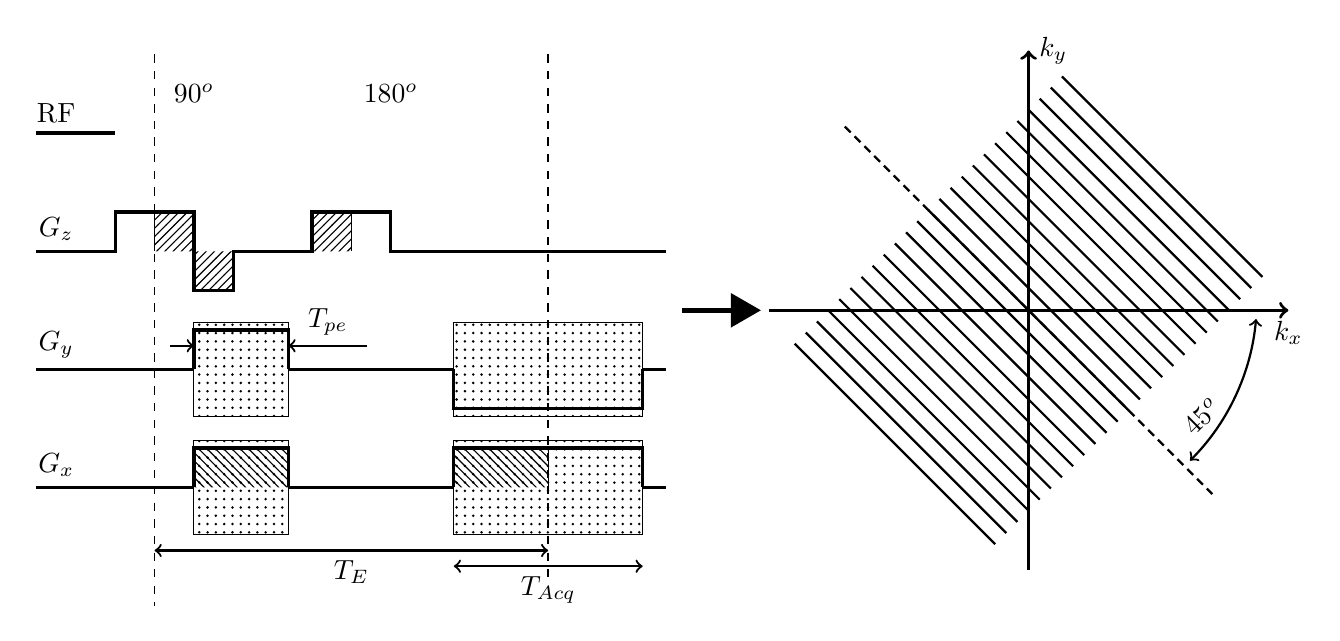
\begin{tikzpicture}[scale=1]
\draw[very thick] (0,0) -- node[near start,above]{RF} (1,0); 
\draw[semithick,dashed] (6.5,1) -- (6.5,-5.7) (1.5,1) -- (1.5,-6);
\pgftransformxshift{1.5cm}
\draw[very thick] plot[smooth] file {sincsmall.txt} -- (2,0);
\node at (0.5,0.5) [] {$90^o$};
\pgftransformxshift{2.5cm}
\draw[very thick] plot[smooth] file {sinc.txt} -- (4,0);
\node at (0.5,0.5) [] {$180^o$};
\pgftransformshift{\pgfpoint{-4cm}{-1.5cm}}
\draw[very thick] (0,0) -- node[near start,above]{$G_z$} (1,0) 
-- (1,0.5) -- (2,0.5) -- (2,-0.5) -- (2.5,-0.5) -- (2.5,0) 
-- (3.5,0) -- (3.5,0.5) -- (4.5,0.5) -- (4.5,0) -- (8,0);
\filldraw[pattern=north east lines] (1.5,0) 
-- (1.5,0.5) -- (2,0.5) -- (2,-0.5) -- (2.5,-0.5) -- (2.5,0) (3.5,0) -- (3.5,0.5) -- (4,0.5) -- (4,0);
\pgftransformshift{\pgfpoint{0cm}{-1.5cm}}
\draw[very thick] (0,0) -- node[near start,above]{$G_y$} (1,0) -- (2,0) (3.2,0) -- (5.3,0) (7.7,0) -- (8,0);
\draw[very thick] (2,0) -- (2,0.5) -- (3.2,0.5) -- (3.2,0) (5.3,0) -- (5.3,-0.5) -- (7.7,-0.5) -- (7.7,0);
\filldraw[pattern=dots] (2,-0.6) rectangle (3.2,0.6) (5.3,-0.6) rectangle (7.7,0.6);
\draw[thick,->] (1.7,0.3) -- (2,0.3);
\draw[thick,->] (4.2,0.3) -- node[midway,above]{$T_{pe}$} (3.2,0.3);
\pgftransformshift{\pgfpoint{0cm}{-1.5cm}} 
\draw[very thick] (0,0) -- node[near start,above]{$G_x$} (1,0) -- (2,0) (3.2,0) -- (5.3,0) (7.7,0) -- (8,0);
\draw[very thick] (2,0) -- (2,0.5) -- (3.2,0.5) -- (3.2,0) (5.3,0) -- (5.3,0.5) -- (7.7,0.5) -- (7.7,0);
\filldraw[pattern=dots] (2,-0.6) rectangle (3.2,0.6) (5.3,-0.6) rectangle (7.7,0.6);
\filldraw[pattern=north west lines] (2,0)
-- (2,0.5) -- (3.2,0.5) -- (3.2,0) (5.3,0) -- (5.3,0.5) -- (6.5,0.5) -- (6.5,0);
\draw[thick,<->] (5.3,-1) -- node[midway,below]{$T_{Acq}$} (7.7,-1);
\draw[thick,<->] (1.5,-0.8) -- node[midway,below]{$T_{E}$} (6.5,-0.8);
\pgftransformshift{\pgfpoint{8.2cm}{2.25cm}} 
\draw[-triangle 60,line width=2pt] (0,0) -- (1,0);
\pgftransformshift{\pgfpoint{4.4cm}{0cm}}
\draw[very thick,->] (-3.3,0) -- (3.3,0) node[anchor=north]{$k_x$};
\draw[very thick,->] (0,-3.3) -- (0,3.3) node[anchor=west]{$k_y$};
\pgftransformrotate{-45}
\draw[densely dashed,thick] (-3.3,0) -- (3.3,0);
\foreach \y in {-2.4,-2.2,...,2.4} \draw[thick] (-1.8,\y) -- (1.8,\y);
\draw[thick,<->] (2.8,0.1) arc (0:40:2.9) node[rotate=45,near start,above]{$45^o$};
\pagebreak
\end{tikzpicture}
\end{center}
\end{ssection}
\end{document}